
% Titlepage

\thispagestyle{empty}
\tolerance=6000

\vspace{1cm}
\begin{center}
{\Huge \bf NBODY6++}\\[0.7cm]
{\Huge  Manual for the Computer Code}\\[0.5cm]
{\Large \textcolor{red}{ATTENTION, WORK IN PROGRESS!\\[0.5cm]
This manual is continously changing and updated.}} \\ 
\end{center}



\vspace{1cm}
\noindent
%
\begin{center}
{\Large Original authors:\\
Emil Khalisi, Long Wang, Rainer Spurzem$^\star$ \\[1ex]
}

{\Large Current main contributors:\\
Francesco Flammini Dotti, Kai Wu, Rainer Spurzem$^\star$ \\[1ex]
}
{\it
$^\star$Astronomisches Rechen--Institut,
M\"onchhofstr. 12--14, 69120 Heidelberg, Germany \\
$^\star$National Astronomical Observatories,  Chinese Academy of Sciences, Beijing, China\\
$^\star$Kavli Institute for Astronomy and Astrophysics,
Peking University, Beijing, China
}\\[1ex]
Contacts:\\
spurzem@ari.uni-heidelberg.de, spurzem@nao.cas.cn \\
fmfd@uni-heidelberg.de \\ Kai.Wu19@student.xjtlu.edu.cn
\end{center}



\noindent
\begin{figure}[bh]
  \centering
  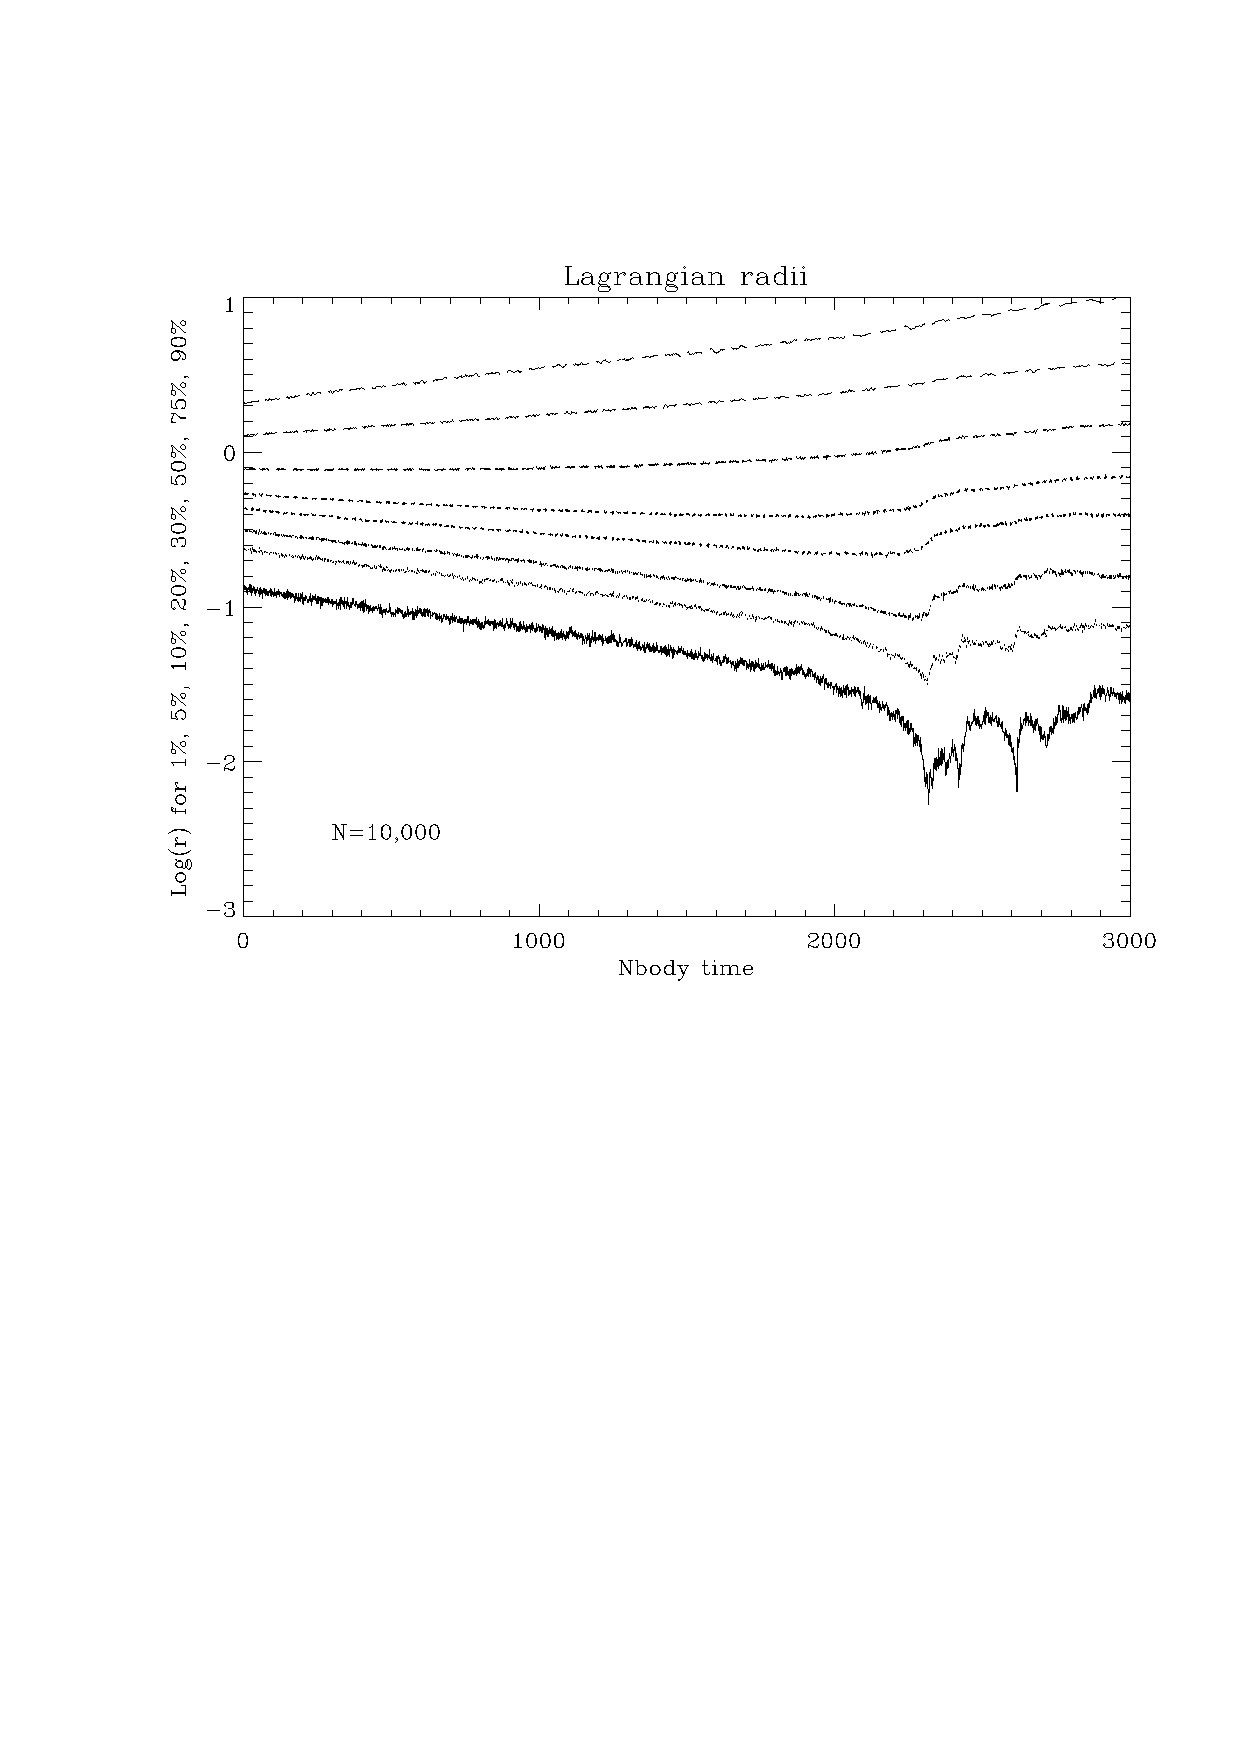
\psfig{figure=eqmass10k_03.pdf,width=0.6\textwidth}
\end{figure}

\noindent
%
\begin{center}

{\it Latest update: \today}
\end{center}
\noindent

\setlength{\headheight}{13.6pt}
\addtolength{\topmargin}{-1.59999pt}

\cleardoublepage


%%%%%  Table of contents

\thispagestyle{fancy}
\renewcommand{\contentsname}{Table of contents}
%\renewcommand{\sectionmark}[1]{\markboth{#1}{}}
\lhead[\itshape \thepage]{\itshape \contentsname}
%\rhead[\itshape \contentsname]{\itshape \thepage}
\cfoot{}

% Table of Contents
\tableofcontents

%%%%% End of introductory pages.


\clearpage

%%%%% Restore previous Header as defined in >broschure.tex<

\pagestyle{fancy}
\renewcommand{\sectionmark}[1]{\markboth{\thesection\ \, #1}{}}
\renewcommand{\subsectionmark}[1]%
                        {\markright{\thesubsection\ \, #1}{}}

\lhead[\itshape \thepage]{\itshape \rightmark}
\rhead[\itshape \leftmark]{\itshape \thepage}
\cfoot{}

